\documentclass[11pt]{standalone}

\usepackage{ifthen}
\usepackage{tikz} 
\usetikzlibrary{shapes.misc}
\usetikzlibrary{arrows,arrows.meta}
\usetikzlibrary{calc,intersections, patterns, math}

\definecolor{pfeil}{RGB}{168,167,167}
\definecolor{petrol}{RGB}{0, 118, 136}
\definecolor{darkgoldenrod}{RGB}{184, 134, 11}
\colorlet{petrol-lighter}{petrol!40}
\colorlet{darkgoldenrod-lighter}{darkgoldenrod!40}

\begin{document}

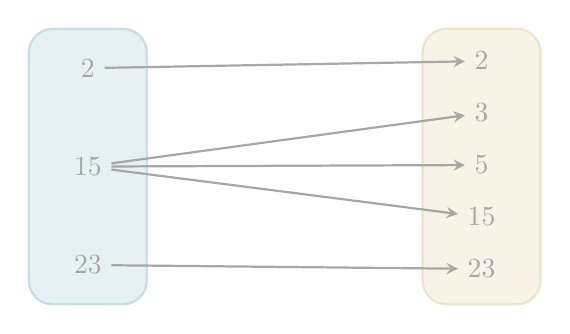
\begin{tikzpicture}[pfeil]

    \draw[thick, fill=petrol!20, draw=petrol-lighter, rounded corners=2ex, opacity=0.5] (0,0) rectangle ++ (1.5,3.5);
    \draw[thick, fill=darkgoldenrod!20, draw=darkgoldenrod-lighter, rounded corners=2ex, opacity=0.5] (5,0) rectangle ++ (1.5,3.5);



				\foreach \x/\y in {1/2, 2/15, 3/23}{
					\node (D\x) at (0.75,4.25-1.25*\x) {\y};
			}
				\foreach \x/\y in {1/2,2/3,3/5,4/15,5/23}{
					\node (Z\x) at (5.75,3.75-0.66*\x) {\y};
			}
				\draw[thick,-stealth] (D1) -- (Z1);

				\foreach \x in {2,...,4}
				\draw[thick,-stealth] (D2) -- (Z\x);

				\draw[thick,-stealth] (D3) -- (Z5);

\end{tikzpicture}

\end{document}